\documentclass[DD.tex]{subfiles}
\begin{document}
\section{Architectural design}
\subsection{Overview: High-level}

The system is going to be implemented with a three tier architecture. \newline Tiers are briefly described by the following schemas.

\begin{figure}[h!]
	\centering
	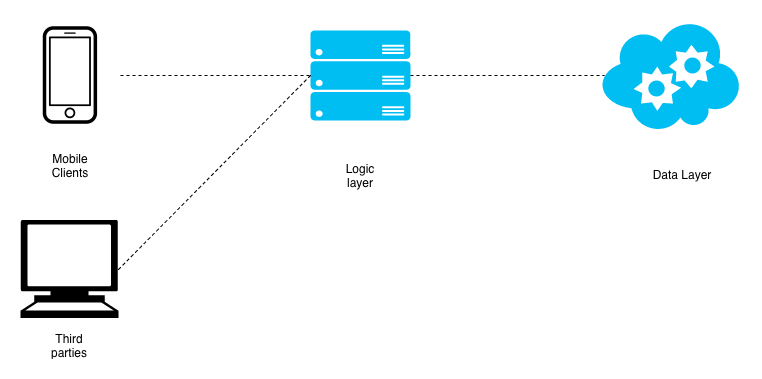
\includegraphics[height=6.00cm,keepaspectratio]{Figures/GeneralSchema}
	\caption{High level view of the system's architecture}
\end{figure}

The decision behind this kind of architecture has been taken in order to build the system in the most modular possibile way. Here is described the organisation of the layers: 

\begin{itemize}
	\item \textit{Presentation layer}:\begin{itemize}
			\item {Individuals}: an iOS application which contains a view of the entire system;
			\item {Third-parties}: a web interface to access to own private profile and find the endpoints to communicate with for acquiring the information of interest.
			\end{itemize}
	\item \textit{Logic layer}: logic layer will implement all the logic of the entire system and will handle communications between clients' app and the data layer.
	\item \textit{Data layer}: data layer will be implemented in third-party's cloud system and will keep persistent users' data.
\end{itemize}

The idea is to keep as separate as possibile the logic layer from the data layer in order to let the system grows in a modular fashion and let us change cloud data provider following the system growth with the minimum effort.

\newpage
\begin{figure}[h!]
	\centering
	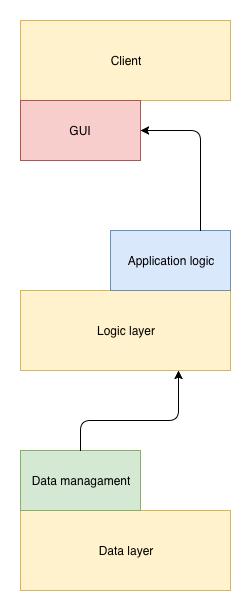
\includegraphics[height=8.00cm,keepaspectratio]{Figures/ThreeTierSchema}
	\caption{Distribution of application's function among the tier}
\end{figure}
\newpage

\subsection{Component view}
We now provide a high level view of system's components. The system is composed by two client components: \textit{Web Interface} and \textit{Mobile Application}; they consume services offered by a set of logic components: \textit{HealthSharing manager}, \textit{SOS manager}, \textit{RunEvent Manager} and \textit{Access Manager}. Each of them will be interfaced with the \textit{DatabaseLink Manager} which provides transparent access to the tier devoted to persistency. \newline We are now going to provide further details of each subsystem.

\begin{figure}[h!]
	\centering
	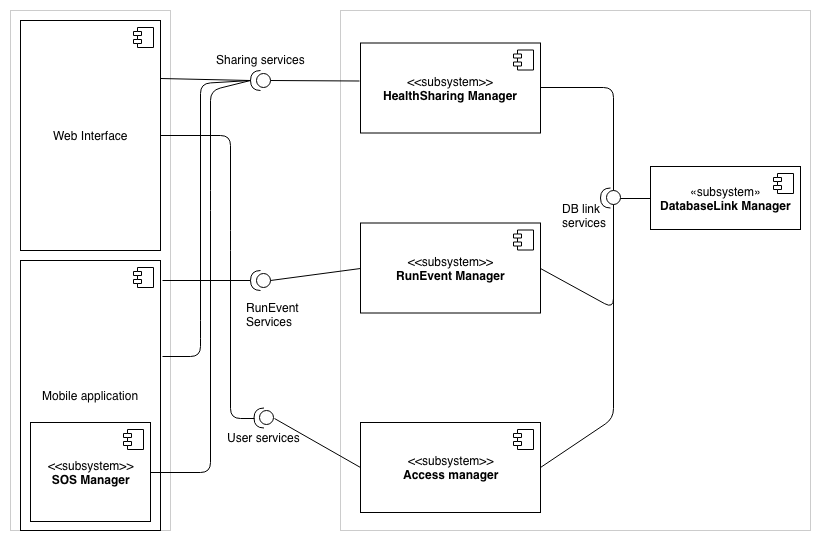
\includegraphics[height=8.00cm,keepaspectratio]{Figures/ComponentOverview}
	\caption{High level overview of system components}
\end{figure}

\newpage
\subsubsection{Component view of HealthSharing Manager}
HealthSharing manager is composed of three main submodules: \begin{itemize}
	\item Access Policy Manager Module;
	\item Data Manager Module;
	\item Data Elaboration Module.
\end{itemize}

The \textit{Access Policy Manager Module} works as a manager of all the policies associated with data sharing. It provides the list of active sharing to users and it let them manage active policies such as accepting new sharing request or change/delete active policies.\\
The \textit{Data Manager Module} has to handle all the operations of retrieving/storing data between users' app and databases. It also has to guarantee data consistency in the whole system.
	\\
The \textit{Data Elaboration Module} has to handle the operations devoted to  data anonymisation and manage the requests of aggregated data from third-parties.

\begin{figure}[h!]
	\centering
	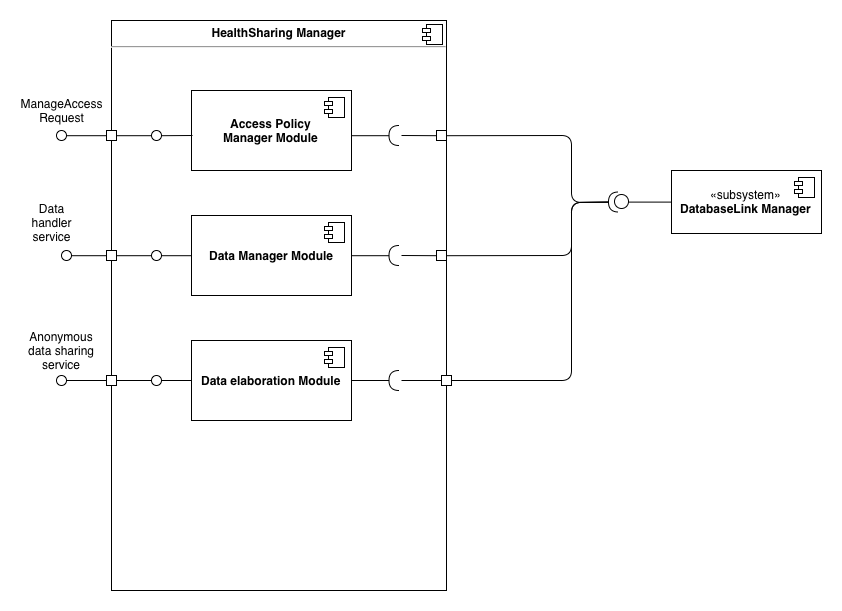
\includegraphics[height=8.00cm,keepaspectratio]{Figures/HealthSharingManagerComponent}
	\caption{Specific description for HealthSharing Manager component}
\end{figure}
\newpage

\subsubsection{Component view of SOS Manager}
The \textit{Anomaly Detection Module} has to read and control heartbeat data from users that have activated SOS functionality in their mobile application. \newline
In case of anomaly, the component activates the routine to handle the emergency cases.
\begin{figure}[h!]
	\centering
	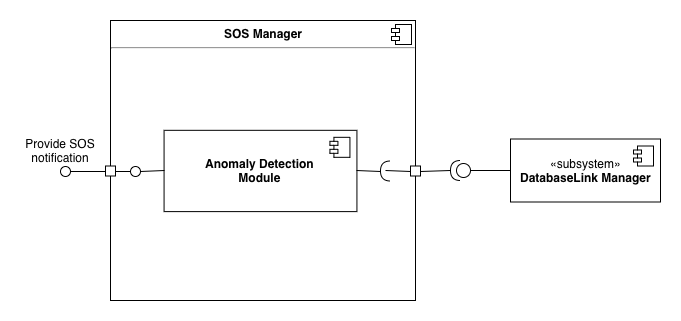
\includegraphics[height=6.00cm,keepaspectratio]{Figures/SOSManagerComponent}
	\caption{Specific description for SOS Manager component}
\end{figure}
\newpage


\subsubsection{Component view of RunEvent Manager}
\begin{figure}[h!]
	\centering
	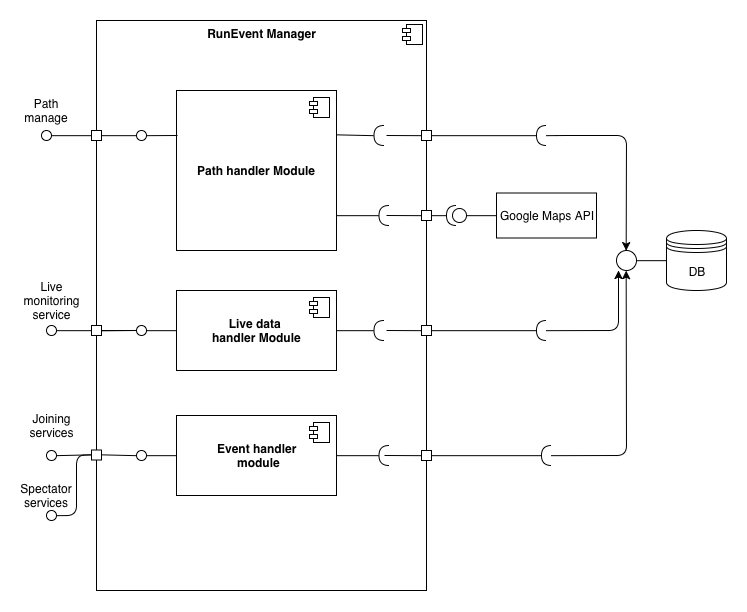
\includegraphics[height=10.00cm,keepaspectratio]{Figures/RunEventManagerComponent}
	\caption{Specific description for RunEvent Manager}
\end{figure}

RunEvent Manager is composed of three main submodules: \begin{itemize}
	\item PathHandler Module;
	\item Live Data Handler Module;
	\item Event Handler module.
\end{itemize}

The \textit{PathHandler Module} has to offer services for creation and paths managing to users. In order to to that, it has to communicate with external map services API.\\
The \textit{Live Data Handler Module} has to handle incoming live data from users and prepare and aggregate them for spectators. Moreover, it has to make them persistent for future access.\\
The \textit{Event Handler Module} has to handle events creation and users' joining operations.

\newpage
\subsubsection{Component view of Access Manager}
\begin{figure}[h!]
	\centering
	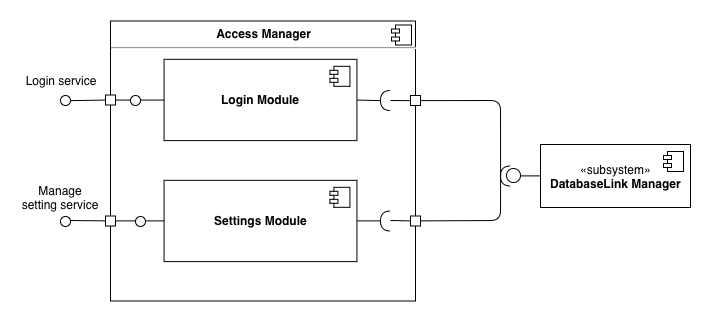
\includegraphics[height=7.00cm,keepaspectratio]{Figures/AccessManagerComponent}
	\caption{Specific description for Access Manager component}
\end{figure}

Access Manager is composed of two main submodules: 
\begin{itemize}
	\item Login Module;
	\item Settings Module.
\end{itemize}

The \textit{Login Module} offers all the function devoted to login for both users and third-parties.\\
The \textit{Settings Module} offers services devoted to let users to change and manage their preferences.



\newpage
\subsubsection{Entity Relationship diagram}
In this section we show the Entity Relationship schema of the adopted DB.
\begin{figure}[h!]
	\centering
	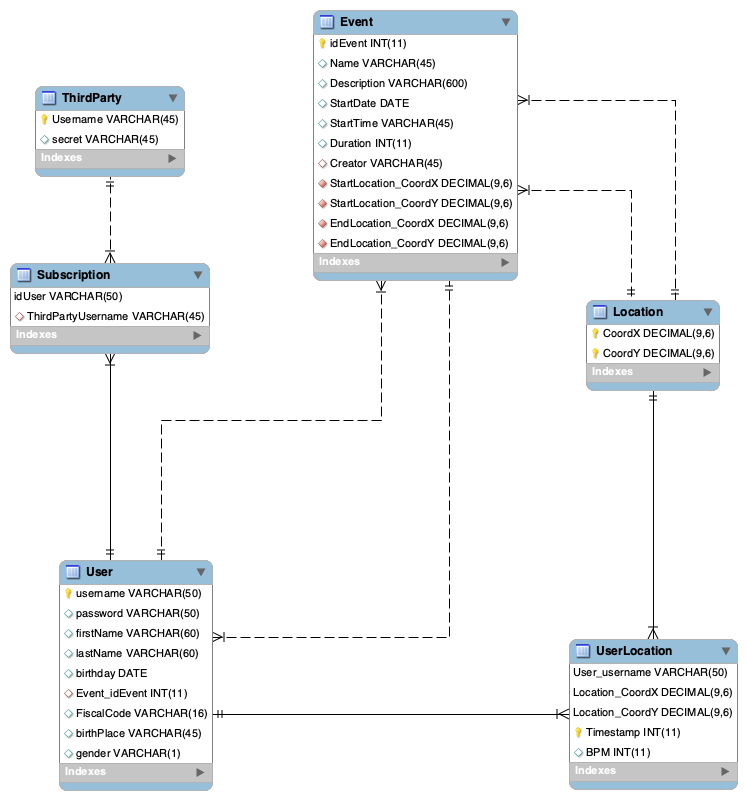
\includegraphics[height=12.00cm,keepaspectratio]{Figures/er-schema}
	\caption{ER schema}
\end{figure}


\newpage
\subsection{Deployment view}

\begin{figure}[h!]
	\centering
	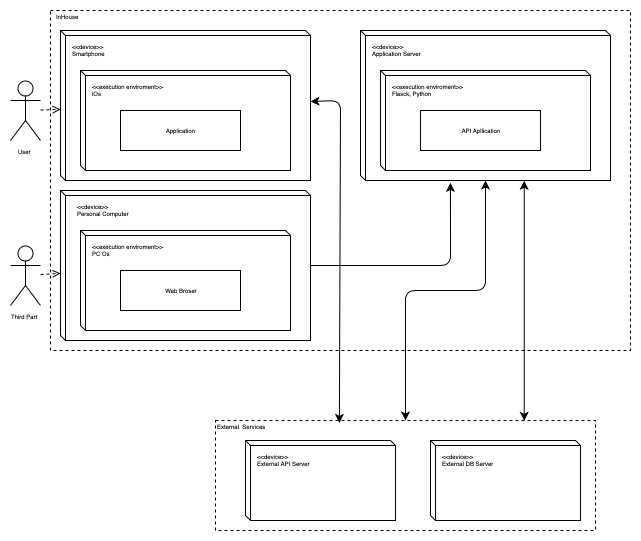
\includegraphics[height=10.00cm,keepaspectratio]{Figures/DeploymentDiagram}
	\caption{Deployment diagram}
\end{figure}

The Deployment diagram emphasises the nodes on which the platform runs;\\
\textbf{InHouse} box represents the components developed inside the company while 
the components in the \textbf{External} box are on-demand softwares.\\
\begin{itemize}
\item	\textbf{Smartphone}: the application deployed on the iOS smartphone used by individuals. Users are able to retrieve data from the application server and also from external APIs directly;
\item \textbf{Web Browser API Interface}: a web page for third-parties registration. It provides a secret to do a request to the API Server;
\item \textbf{Application Server}: the  main logic core of the application. It’s the only access point to the DB but it also communicates with the external server API;
\item  \textbf{External Services}: both the external services are represented as  blackboxes because we don't know how they are implemented.
\end{itemize}
\newpage

\subfile{"RunTimeview.tex"}	
	
\newpage
\subsection{Component interfaces}
\begin{figure}[h!]
	\centering
	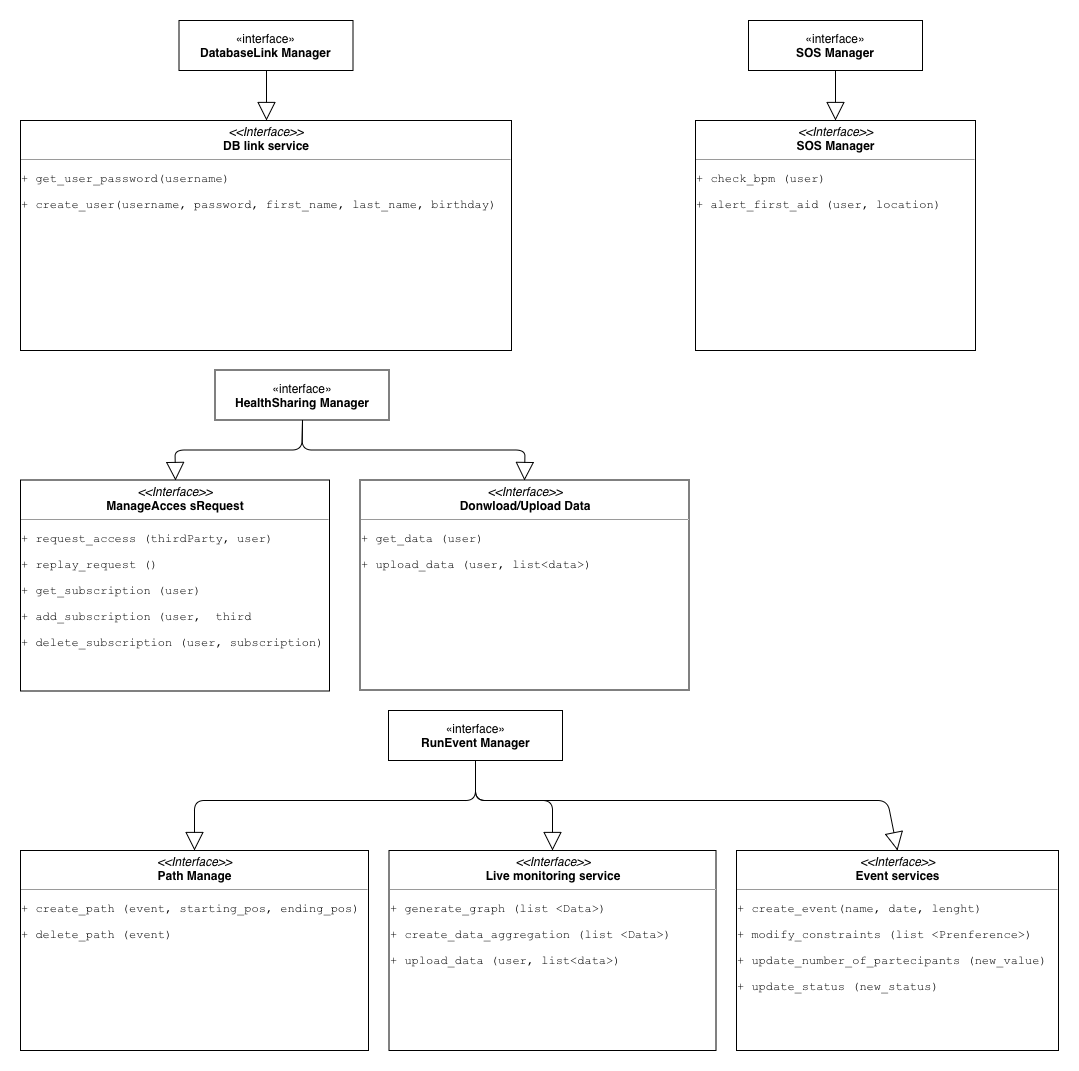
\includegraphics[height=16.00cm,keepaspectratio]{Figures/Interfaces}
	\caption{Components' interfaces descriptions diagram}
\end{figure}



\newpage

\subsubsection{API structure}
The whole Data4Help infrastructure will be connected through a RESTful API system. JSON files will be used as serialisation data format.\\
All the API system will be implemented referring to a single endpoint (www.data4help.cloud) that TrackMe organisation will buy for the implementation of this project.
\\Users' applications and third-parties will refer to different subdomain:

\begin{itemize}
	\item \textit{\textbf{www.data4help.cloud/api/users}}: it will be the specific endpoint for the application that serves users;
	\item \textit{\textbf{www.data4help.cloud/api/thirdparties}}: it will be the specific endpoint for third-parties.
\end{itemize}

Secure access will be provided by HTTPS Basic Access Authentication: each request between client and server will be authenticated with user/third-party credential.

Here a complete description of each supported methods:

\begin{itemize}

	\item \textit{\textbf{/api/user/registration}}
		\begin{itemize}
			\item POST: register a new user with credentials specified in HTTP fields;
		\end{itemize}
	\item \textit{\textbf{/api/user/data}}
		\begin{itemize}
			\item GET: get last fixed number user's data;
			\item POST: upload new user's data;
		\end{itemize}
	\item \textit{\textbf{/api/user/request}}
		\begin{itemize}
			\item GET: get all access requests that have the user as target;
		\end{itemize}
	\item \textit{\textbf{/api/user/request/\{request\_id\}}}
		\begin{itemize}
			\item PUT: accept or deny the request with the given ID;
		\end{itemize}
	\item \textit{\textbf{/api/thirdparties/registration}}
		\begin{itemize}
			\item POST: register a new third-party with credentials specified in HTTP fields;
		\end{itemize}
	\item \textit{\textbf{/api/thirdparties/request}}
		\begin{itemize}
			\item POST: generate a new access request for a user's data;
		\end{itemize}
	\item \textit{\textbf{/api/thirdparties/data}}
		\begin{itemize}
			\item GET: update all data coming from subscribed user.
		\end{itemize}
\end{itemize}


\newpage
\subsection{Selected architectural styles and patterns}
Data4Help system is based on a tree tier architecture:
\subsubsection{Overall Description}
\begin{itemize}
	\item \textbf{Presentation Tier} has to present the data to the user in such a way that they are meaningful for the user's perspective. It displays information obtained communicating with the other two tiers. For example, if a user performs a tap on the button "Create new run event", the presentation tier sends a request to the Logic Tier that will answer with a message requiring information to create the event and so on.
		To be quick to react in case of “Anomaly detection”, instead of putting the logic of continuous checking of the vital parameters into the Logic Tiers (as the entire logic of the application) the Presentation Tier (the application) contains also this component. Doing this we will be able to speedy react and call the ambulance in the quickest way possible. We are also able to react in narrow situation as absence of field coperture or not working internet network.
	\item \textbf{Logic Tier} has the entire logic needed for the application (excluding the “Anomaly detection” component as described above). It receives the requests from the Presentation Tier and, if needed, queries the Data tier before sending back replies.
	\item \textbf{Data Tier} is composed of a DBMS that provides an interface to the DataBase externally located. It contains all the data in a Relational Schema (ER) (view Figure 8)\\\\
	The separation between the different layers allow us to upgrade or replace a single tier without affecting the others.
\end{itemize}
\subsubsection{Design Patterns}

\begin{itemize}
	\item \textbf{Model View Controller (MVC)}\\\\
		\textbf{MVC in a nutshell}\\\\
		The MVC is an architectural pattern that permits to separate the presentation layer of the application from the business logic layer. It is composed by the following layers: \\
		\vspace{-5mm}
		\begin{itemize}
		\setlength\itemsep{-0.9em}
			\item\textbf{Model}: the section that contains only the data of the application;\\
			\item\textbf{View}: the section that contains the component needed to represent information;\\
			\item\textbf{Controller}: the section that contains the logic of the application; it maps the user's input coming from the View to make changes to the Model section.\\
		\end{itemize}
		\newpage
	\item \textbf{MVC in Data4Help}\\\\
		In Data4Help application the \textbf{Model} is the persistent data storage layer with the relational SQL Database (view section 2.2.5) placed externally.\\
		The \textbf{View} is the application displayed on the user's smartphone; is the only point of interaction with the client.
		This component contains the "UI Controller" that is the logic that handles the events on the UI. It also contains the logic of AutomatedSOS as explained in the above sections.\\
		The \textbf{Controller} is placed on the web server and is accessible with the RESTful API. It contains the logic of the application.\\
\end{itemize}

\subsubsection{Other design decision}
We decided not to let logic components directly deal with the database but to interleave the \textit{DatabaseLink Manager} in order to build the logic layer independently from the persistent layer. Developers will be able to change the way the system interacts with the database or to change database's interfaces without having to change all the components. \\\\
Another important design decision the team has taken is not to operate directly with wearable devices but instead to rely on mobile OS' features to acquire data. In particular: the system is going to take advantage of Apple HealthKit framework to read data. This will let the application communicate with all wearable devices that are already compliant with Apple's framework without having to be compliant with each vendor's specific device.
\end{document}